\section{Test cases for complex statecharts: orthogonality}
\label{testOrthogonality}

Now we shall consider statecharts that possess orthogonality, in other words, states in concurrent regions.

One fisrt method to generate test cases dealing with orthogonality is to eliminate it by flattening the statechart as explained in \ref{flattening}. The elimation of orthogonality would be done with the cartesian product of all states and transitions causing an explosion in the number of result states and transitions \cite{bogdanov}.

To avoid state and transition explosion and still be able to cover all states and test all transitions, \cite{bogdanov} offers the alternative to refine the concurrency requisites. In this project, we chose the strong concurrency refinement:

\begin{itemize}

\item \textbf{Strong concurrency}

This refinement allows us to test concurrent components separately. Transitions from each concurrent region are triggered one-by-one in different steps. In this case, we consider that the concurrent regions are placed in units which either run in parallel or in different processors. So no concurrent region may cause missing transitions in another one or misdirected transitions.
\end{itemize}

The communication resources, as broadcasting, should be disabled during testing since it could cause series of transitions to occur. A chain reaction would be an example of such series and would not be expected by the test cases listed using this implementation.

We first compute the coverage paths for each concurrent region separately. Then, similarly to the case with hierarchy, we combine these paths with the coverage path of the state that contains the concurrent regions. After obtaining the coverage path for all states, set $C$ is complete. 

In the next pseudocode, we consider that substates are in a region inside the superstate. To apply the next pseudocode for statecharts with hierarchy discussed in the previous section (\ref{testHierarchy}) we should consider that the superstate have only one internal region, which will contain the substates. In statecharts with concurrency, the concurrent elements would be in different regions inside a superstate; figure \ref{fig:stockUpdateEmail} serves as an example. Therefore, the solution can be applied to states with orthogonality as well as to ones with hierarchy only. Find below the pseudocode for the contruction of the \textit{State Cover} set, set $C$:

\begin{lstlisting}[mathescape,label={testOrthogonalityPseudo}]
//Recursive function that will do all the work
//returns the State Cover set, or set C
Set constructSetCRec(State s, Path p, Set setC, List visited) {

	visited.add(s);

	setC.add(s,p);

	if (s.containsSubRegions()) {

		for (Region r in s.getSubregions()) {
			
			Set subSetC = constructSetC(r.getInitialSubstate());	

			r.addSubpaths(subSetC);

			setC.remove(s,p);

			for (State substate in s.getSubstates()) {
	
				Path partialPath = subSetC.getPath(substate);
	
				Path substateCoveragePath = p + partialPath;
	
				setC.add(substate,substateCoveragePath)	
			}
		}	
		
	}
	
	for (Transition t in s.getOutgGoingTransitions()) {
		
		State nextState = t.getDestiny();

		if (!visited.contains(nextState)) {

			if (s.containsSubstates()) {
			
				Path nextCoveragePath = p + $\Delta_{s}$ + t.getLabel());

			} else {

				Path nextCoveragePath = p + t.getLabel());

			}	

			constructSetCRec(nextState,nextCoveragePath,setC,visited);	
		}
	}
	
	return setC;
}
\end{lstlisting}

Next, we again need to generate the test cases for each transition of the model. This process is the same as the one described in the case with hierarcy since concurrent states are inside a super state. The algorithm for this phase can be found in pseudocode format in \ref{pseudocodeTestCase}.

\begin{figure}[htb]
\centering
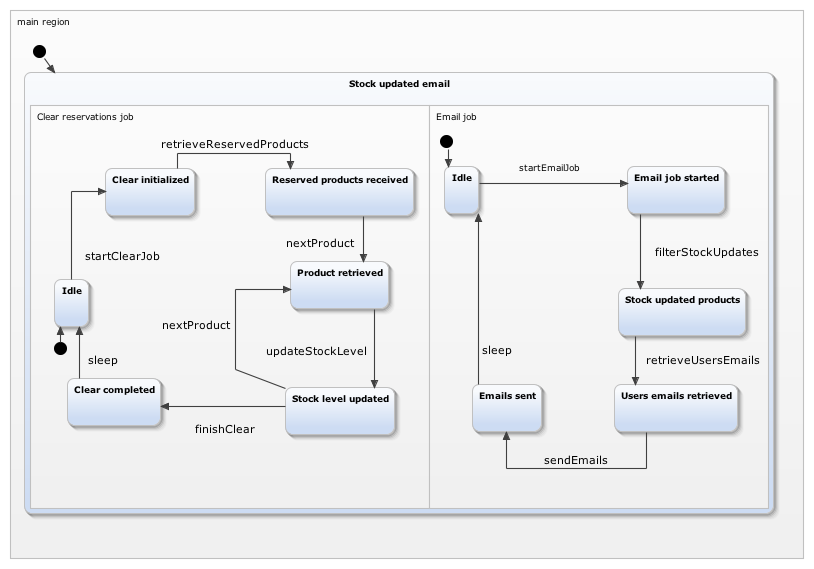
\includegraphics[width=15cm]{figuras/stockUpdateEmail}
\caption{\label{fig:stockUpdateEmail} Statechart model for concurrent jobs: clear reservations job and send email job}
\end{figure}

To ilustrate this case, we can look at the example provided in figure \ref{fig:stockUpdateEmail}. It models an online store in which the administrator is allowed to execute two jobs: one to clear all reservations in every product (region \textit{Clear reservations job} in the figure) and one to send emails to customers letting them know certain products are back in stock (region \textit{Email job} in the figure). Both jobs can run in parallel if the administrator whishes, thus their regions are modeled in a concurrent way in the statechart. 

According to our refinement, the coverage paths will be created for substates in \textit{Clear reservations job} and \textit{Email job} separately. First, the substates in \textit{Clear reservations job} concurrent region are inside state \textit{Stock update email}, hence we need to apply the algorithm presented in \ref{testOrthogonalityPseudo}. Note that since the coverage path to \textit{Stock update email} is just the empty string $e$, it will not have a great impact in the substates paths. Let's consider \textit{Product retrieved} and \textit{Stock level updated} to exemplify the results:

\begin{center}
\begin{tabular}{| p{4cm} | p{10cm}|}

\hline

State & Coverage path \\ \hline

Product retrieved & e e startClearJob retrieveReservedProducts nextProduct \\ \hline

Stock level updated & e e startClearJob retrieveReservedProducts nextProduct updateStockLevel \\

\hline
\end{tabular}
\end{center}

Secondly, we can construct the coverage paths for substates in region \textit{Email job} by an analogous process. For instance, the coverage path for \textit{Email sent} would be:

\begin{center}
\begin{tabular}{| p{4cm} | p{10cm}|}

\hline

State & Coverage path \\ \hline

Email sent & e e  startEmailJob filterStockUpdates retrieveUsersEmails sendEmails\\ 
\hline
\end{tabular}
\end{center}

The generation of the test cases, then, is similar to the one presetend in the previous section (\ref{testHierarchy}). But, when there is orthogonality, we need to consider the coverage paths of substates from all concurrent regions in a state during the expansion phase. For the example in \ref{fig:stockUpdateEmail}, because we do not have a state after \textit{Stock updated email}, no expansion of coverage paths will be needed.

To demonstrate, we will consider the test cases for transitions \textit{nextProduct}, from state \textit{Stock level updated}, and \textit{sleep}, from state \textit{Email sent}. We need to concatenate these transition labels to the end of the coverage path of their origin state. Therefore, \textit{nextProduct} will be appended to the coverage path of \textit{Stock level updated} and \textit{sleep}, to the coverage path of \textit{Email sent}:

\begin{itemize}

\item Test case for \textit{\textbf{nextProduct}}

Path: \textit{e e startClearJob retrieveReservedProducts nextProduct updateStockLevel nextProduct}

Expected state: \textit{Product retrieved}

\item Test case for \textit{\textbf{sleep}}

Path: \textit{e e  startEmailJob filterStockUpdates retrieveUsersEmails sendEmails sleep}

Expected state: \textit{Idle}

\end{itemize}
